\chapter{Testovanie a vyhodnocovanie}
\label{chap:testovanie-vyhodnocovanie}
Po naimplementovaní navrhnutého riešenia, ktoré bolo popísané v kapitole \ref{chap:implementacia}, nasledovalo testovanie a vyhodnocovanie, ktorému sa venuje práve táto kapitola.  Kapitola začína popisom testovania serverového aplikačného riešenia pomocou testovacieho rámca Tavern, pokračuje testovaním užívateľského rozhrania aplikácie a vyhodnocovaním naimplementovanej detekcie chronických rán. Na záver kapitoly sú zhrnuté ďalšie možné vylepšenia práce a je načrtnuté budúce smerovanie projektu. 

%%%%%%%%%%%%%%%%%%%%%%%%%%%%%%%%%%%%%%%%%%%%%%%%%%%%%%%%%%%%%%
\section{Testovanie serverového aplikačného rozhrania}
Testovanie aplikačného rozhrania prebiehalo už počas samotnej implementácie, kedy vždy po naprogramovaní nejakej sady koncových adries, boli napísané aj testy na overenie funkcionality týchto adries. Testovanie prebiehalo pomocou Python testovacieho rámca Tavern, ktorý je voľne dostupný pod licenciou MIT. Tavern je plugin pre Pytest, nástroj príkazovej riadky a aj Pythonova knižnica v jednom určená pre testovanie aplikačných rozhraní založených nielen na RESTe. Používa syntax založenú na YAML, ktorá je veľmi flexibilná a jednoduchá. Okrem RESTful aplikačných rozhraní dokáže testovať aj rozhrania založené na MQTT. Veľká výhoda Tavern je, že môže byť veľmi jednoducho použitý v hocijakom continous integration procese. \cite{AXUaooptJGOSpUrX} 

Testy vytvorené pre Tavern sú teda definované v YAML súboroch, ktoré predstavujú danú testovaciu sadu. Táto sada je vždy definovaná svojím menom (\textit{test\_name}) a jednotlivými krokmi samotného testu (\textit{stages}).  Každý jeden krok predstavuje samostatné dotazovanie sa na server a volanie serverovej funkcie. Kroky sa skladajú z mena kroku (\textit{name}), z požiadavky (\textit{request}), ktorá sa vykonáva a z odpovede (\textit{response}), ktorá sa kontroluje. V požiadavke je možné definovať všetky nastavenia, ako url adresy serveru (\textit{url}), na ktorý sa bude posielať požiadavka, metódu, ktorá sa bude vykonávať (\textit{method}), dáta vo formáte json, ktoré sa na server budú odosielať (\textit{json}) a prípadne ďalšie hlavičky (\textit{headers}), ktoré sú v požiadavke prítomné (v tomto prípade je prítomná iba hlavička \textit{Authorization}). Správnosť odpovede, ktorá sa potom vyhodnocuje je overovaná podľa vráteného stavového kódu (\textit{status\_code}) a dát obsiahnutých v tele (\textit{body}), poprípade iných položiek, ktoré ale v prípade tejto práce nie sú potrebné. Štruktúru takéhoto kroku testu je možné vidieť pre predstavu v kóde. 
\begin{lstlisting}[caption={Ukážka testovacieho kroku.},captionpos=b]
...
- name: Get scale list after update
    request:
      url: "{env_host:s}/scale"
      method: GET
      headers:
        Authorization: "{firebase_token:s}"
    response:
      status_code: 200
      body:
        - name: Scale
          unit: px
          value: 10
          user: "{firebase_user:s}"
          _id:
            \$oid: "{scale_id:s}"
...
\end{lstlisting}
Testy sú spúšťané pomocou nástroju príkazového riadku Tavern-CI. Testy tejto práce boli rozdelené do 2 súborov, a to na prípady, ktoré môžu nastať pri každodennom používaní aplikácie (\textit{valid.tavern.yaml}) a na prípady, ktoré by mohli nastať iba v prípade nejakej neočakávanej chyby, alebo pri pokuse o hackovanie aplikácie (\textit{invalid.tavern.yaml}). Súbor \textit{enviroment.yaml} slúži na uchovávanie premenných, ktoré sa používajú a sú vkladané do obidvoch testov. Ide o premennú kľúča k Firebase Authentification, e-mailu a hesla k účtu testovacieho užívateľa a koreňovú adresu serveru aplikačného rozhrania. Kroky testu sa vyhodnocujú postupne a v prípade, že sa nevyhodnotí správne jeden krok, tak vyhodnocovanie ďalších krokov je zrušené a užívateľ je o tejto skutočnosti informovaný. Po otestovaní finálnej podoby aplikačného serverového rozhrania, kedy všetky testy dopadli úspešne, bolo toto rozhranie považované za stabilné a fungujúce správne. 

%%%%%%%%%%%%%%%%%%%%%%%%%%%%%%%%%%%%%%%%%%%%%%%%%%%%%%%%%%%%%%
\section{Vyhodnocovanie detekcie chronickej rany}
Vyhodnocovanie a testovanie detekcie bolo vykonávané na snímkoch chronických rán, ktoré poskytla Fakultná nemocnica Brno. Ide o snímky vytvorené pomocu bežnej mobilnej kamery, ktorá nebola ničím špeciálna a nachádza sa takmer v každom modernom mobilnom zariadení. Snímky sú rôznej kvality a zachycujú rôzne chronické rany v rôznom štádií, od rán, ktoré sa skoro neprejavili, až po rany, ktoré už boli v pokročilom štádií a značne komplikované ako na liečbu, tak aj na samotnú detekciu. Snímky boli získavané nemocnicou približne od polovice januára 2018 do polovice mája 2018 a bolo takto možné získať 40 snímok 14 unikátnych defektov (v rovankom čase bol ten istý defekt zachytený niekoľkokrát). Z tých 14 defektov sa avšak nejednalo vždy o chornické rany, ale objavili sa aj starecké škvrny, alebo jendo 60 ročné znamienko. Unikátnych chronických rán bolo teda dokopy 12 a z toho 10 bolo použitých pre vyhodnocovanie. Všetky unikátne rany boli autorom práce anotované pomocou konzultácií s extenrým konzultantom tejto práce.

Samotné vyhodnocovanie a testovanie bolo vykonávané tak, že testovacie snímky boli manuálne ohraničené externým konzultantom z nemocnice pomocou špeciálne vytvorenej webovej aplikácie pre tieto účely. Je nutné podotknúť, že chronické rany sú veľmi zložité a keď sa stretne viacero špecialistov, tak môžu mať rozdielny názor, čo ešte patrí do priestoru rany a čo už rana nieje. Je teda nutné pri detekcií a aj tvobre predlohy vždy rátať s určitou dávkou subjektivity. Rany na snímkach boli potom vždy detekované pomocou poloautomatickej metódy detekcie a manuálnej detekcie. Manuálna detekcia bola vykonaná podľa predlôh. Po detekcií, či už manuálnej alebo automatickej boli hodnoty vypočítaného obsahu rany v pixeloch navzájom porovnávané. Výsledky je možné vidieť v tabuľke \ref{tab:result}, kde je vždy číslo rany, ktoré dopovedá menu súboru z priečinku shots/eval nachádzajúceho sa na CD. Úspešnosť detekcie je vyjadrená číselne, kde hodnota 100\% odpovedá rane, ktorá ja zhodná s predlohou, hodnota pod 100\% znamená, že určité percento pixelov neoblo detekovaných a hodnota nad 100\% zase hovorí o tom, že určité percento pixelov bolo detekovaných nad rámec.
\begin{table}[h]
\centering
\label{tab:result}
\begin{tabular}{|l|l|l|l|}
\hline
Rana & Automatická detekcia (px) & Očakávaná hodnota (px) & Miera zhody (\%) \\ \hline
1    & 6889                      & 14421                             & 47,77         \\ \hline
2    & 331                       & 619                               & 53,47         \\ \hline
3    & 1538                      & 10830                             & 14,20        \\ \hline
4    & 11073                     & 2648                              & 418,16        \\ \hline
5    & 8415                      & 9071                              & 92,76        \\ \hline
6    & 3724                      & 3137                              & 118,71        \\ \hline
7    & 47603                     & 34756                             & 136,96         \\ \hline
8    & 6788                      & 7683                              & 88,35        \\ \hline
9    & 24654                     & 2703                              & 912,09        \\ \hline
10   & 5914                      & 6969                              & 84,86        \\ \hline
\end{tabular}
\caption{Výsledky vyhodnocovania}
\end{table}
V tabuľke výsledkov je možné si všimnúť, že hodnoty boli rôzne, tak ako jednotlivé rany. Behom práce bolo navrhnuté aby sa projekt zameral len na určitý druh rán v určitom štádií, vzhľadom na to, aké až príliš rozdielne boli jednotlivé rany. Bohužiaľ ale behom pol roka nebolo možné získať taký dostatočný počet snímkov, aby bolo možné sa užšie zamerať. Z obrázkov je jasné, že čo rana to v podstate iný druh v inom štádií, preto boli v rámci implementácie zvolené postupy také aké boli. Z tabuľky je možné si všimnúť hodnoty, ktoré sú až výrazne nad 100\%. Tieto rany boli síce detekované, avšak do okolia rany bol zahrnutý aj predstupeň pred defektom. Takúto ranu je možné vidieť na obrázkoch \ref{fig:w4} a \ref{fig:w4d}. Naopak veľmi dobre boli detekované rany, ktoré boli jasne iné ako okolitá pokožka a aj lajk by dokázal ranu ohraničiť, takým príklaodm môže byť rana na obrázkoch \ref{fig:w8} a \ref{fig:w8d}.
\begin{figure}[h]
   \begin{minipage}{0.48\textwidth}
     \centering
     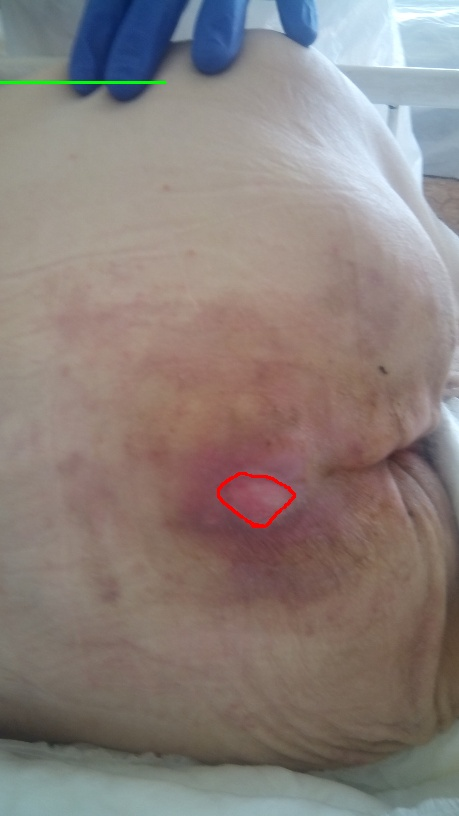
\includegraphics[scale=0.35]{fig/4m.jpeg}
      \caption{Rana 4 - manuálna detekcia, očakávaná.}
      \label{fig:w4}
   \end{minipage}\hfill
   \begin{minipage}{0.48\textwidth}
     \centering
     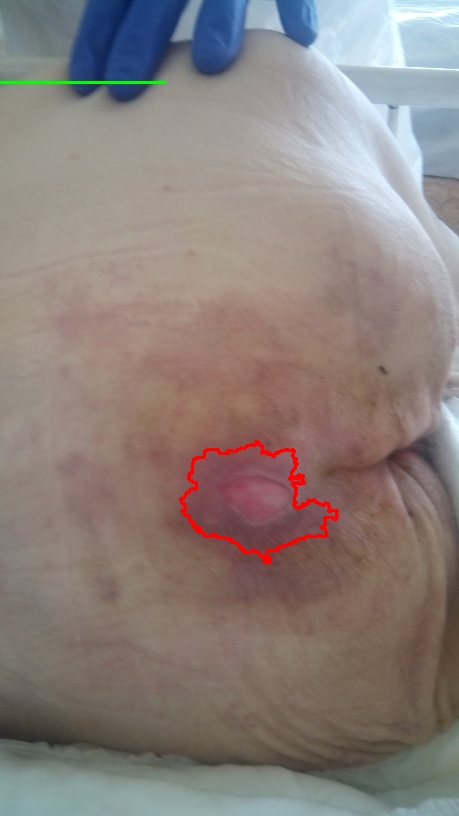
\includegraphics[scale=0.35]{fig/4a.jpeg}
      \caption{Rana 4 - automatická detekcia.}
      \label{fig:w4d}
   \end{minipage}
   \break \break \break
   \begin{minipage}{0.48\textwidth}
     \centering
     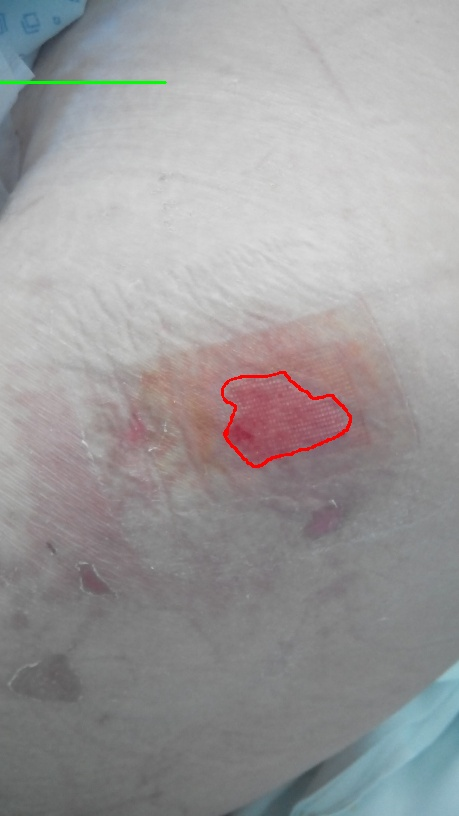
\includegraphics[scale=0.35]{fig/8m.jpeg}
      \caption{Rana 8 - manuálna detekcia, očakávaná.}
      \label{fig:w8}
   \end{minipage}\hfill
   \begin{minipage}{0.48\textwidth}
     \centering
     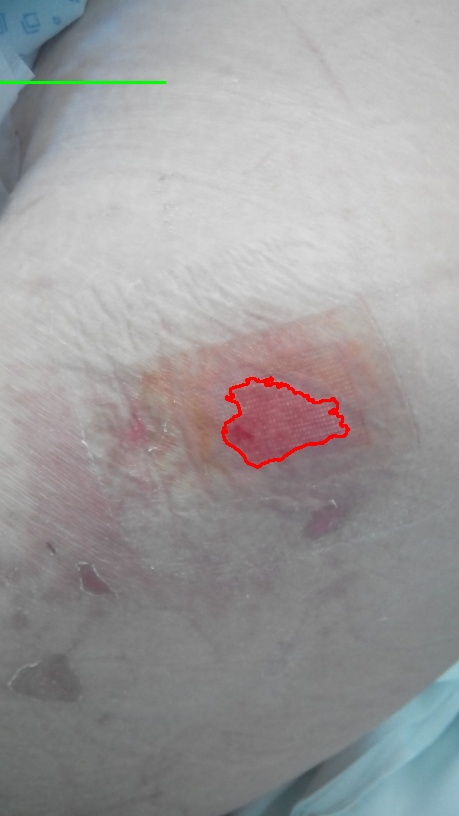
\includegraphics[scale=0.35]{fig/8a.jpeg}
      \caption{Rana 8 - automatická detekcia.}
      \label{fig:w8d}
   \end{minipage}
\end{figure}

%%%%%%%%%%%%%%%%%%%%%%%%%%%%%%%%%%%%%%%%%%%%%%%%%%%%%%%%%%%%%%
\section{Ďalšie smerovanie projektu}
Ako je možné vidieť, tak poloautomatická detekcia funguje rôzne na rôznych snímkach. Zatiaľ čo funguje na ranách, ktoré sú farebne dobre oddelené od okolitej kože, tak pomerne výraznejšie zlyháva na ranách, ktoré sú menej výrazné, alebo sú výrazne komplikované. Avšak aby boli tieto tvrdenia potvrdené, je nutné urobiť ďalšiu a oveľa väčšiu sadu snímkov, a keďže behom 5 mesačného obdobia bolo bolo zaznamenaných 12 unikátnych defektov, typu chronická rana, tak tento proces bude nezanedbateľne časovo trvať. Z toho dôvodu nie je úplne overená funkčnosť poloautomatickej detekcie. Aplikácia avšak môže byť využívaná, tak, že sa bude používať poloautomatická detekcia na jendoduchších a farebne výraznejších ranách, a na zložitejších ranách bude využívaná manuálna detekcia, pomocu ohraničenia rany prstom/myšou. Okrem toho, že poloautomatická detekcia bola testovaná na chronických ranách, tak bola testovaná aj na pár snímkach hematomov a jendom výraznom znamienku, ktoré nemocnica taktiež poskytla. Ako je vidieť na obrázkoch \label{fig:w2} a \label{fig:w3}, tak aplikácia môže byť použitá aj na takéto prípady, poprípade sa môže algoritmus ľahko upraviť, aby mohli byť detekované všetky tieto prípady, keďže hematómy sú v porovnaní s chronickými ranámi oveľa menej rozmanité.
\begin{figure}[h]
   \begin{minipage}{0.4\textwidth}
     \centering
     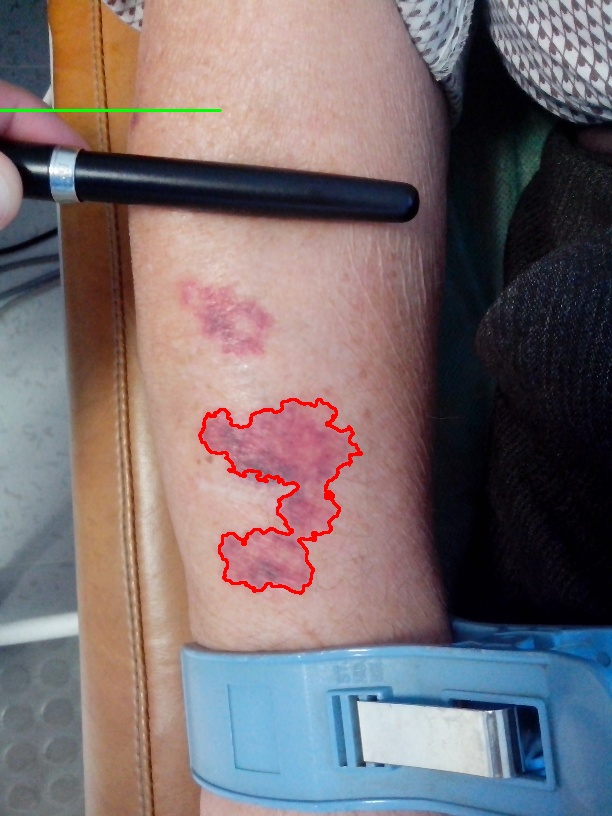
\includegraphics[scale=0.35]{fig/2o.jpeg}
      \caption{Detekcia hematómu.}
      \label{fig:w2}
   \end{minipage}\hfill
   \begin{minipage}{0.4\textwidth}
     \centering
     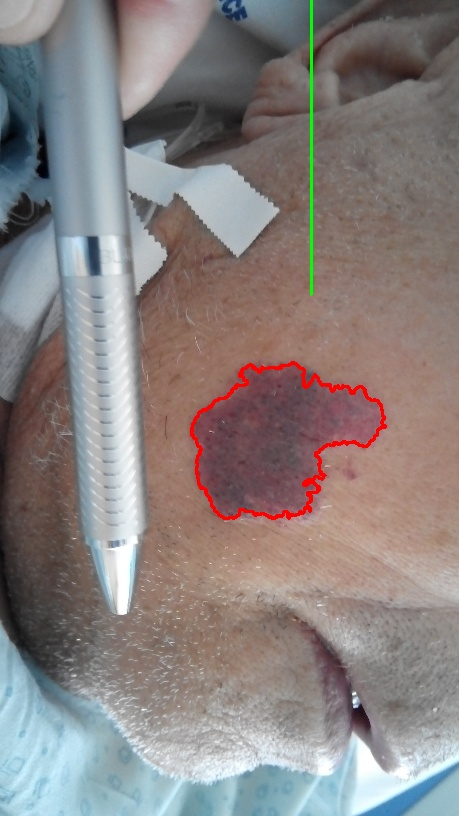
\includegraphics[scale=0.35]{fig/3o.jpeg}
      \caption{Detekcia znamienka.}
      \label{fig:w3}
   \end{minipage}
\end{figure}